\documentclass{article}

% Import packages from local file
\usepackage{packages}

% Define the homework number as a variable
\newcommand{\HomeworkNumber}{8}

\begin{document}

% Add the cover


% Set up custom date format
\newdateformat{monthyeardate}{\monthname[\THEMONTH] \THEYEAR}

% Header and Footer configuration
\pagestyle{fancy}
\fancyhf{}
\fancyhead[L]{\leftmark}
\fancyhead[R]{\thepage}
\fancyfoot[C]{Probabilistic Modeling and Reasoning Homework \HomeworkNumber}

% Chapter and Section formatting
\titleformat{\chapter}[display]
  {\normalfont\bfseries}{}{0pt}{\Huge}
\titlespacing*{\chapter}{0pt}{-20pt}{20pt}

% Adjust header height and top margin
\setlength{\headheight}{14.49998pt}
\addtolength{\topmargin}{-2.49998pt}

% Custom abstract environment
\newenvironment{customabstract}
  {\vspace*{1cm}
   \begin{center}
   \bfseries \huge Abstract
   \end{center}
   \vspace{0.5cm}
   \normalfont \large}
  {\vspace{1cm}}



\makeatletter
% Taken from http://ctan.org/pkg/centernot
\newcommand*{\centernot}{%
  \mathpalette\@centernot
}
\def\@centernot#1#2{%
  \mathrel{%
    \rlap{%
      \settowidth\dimen@{$\m@th#1{#2}$}%
      \kern.5\dimen@
      \settowidth\dimen@{$\m@th#1=$}%
      \kern-.5\dimen@
      $\m@th#1\not$%
    }%
    {#2}%
  }%
}
\makeatother


\begin{titlepage}
    \centering

    % University logo
    \vfill
    
\includegraphics[width=0.3\textwidth]{UOMLOGOEN.eps}
    \vfill

    % Main title
    {\Huge \textbf{Probabilistic Modeling and Reasoning}} \\
    {\LARGE Homework — \HomeworkNumber}

    \vfill  % Vertical fill for dynamic centering
    % Authors' names
    {\Large \textbf{Nikolaos Liouliakis (AID25001)}} \\
    {\Large \textbf{Vasileios-Efraim Tsavalia (AID25006)}}

    % \vfill

    % % Course submission information
    % {\Large A report submitted for the course} \\
    % {\Large \textbf{Probabilistic Modeling and Reasoning}}

    \vfill

    % Program and University information
    {\Large MSc in Artificial Intelligence and Data Analytics} \\
    {\Large University of Macedonia}

    \vfill


    % Supervisor information
    {\Large \textbf{Supervisor: Professor Dimitris Christou-Varsakelis}}

    \vfill

    % Date with custom format
    {\Large \monthyeardate\today} % Automatically displays in "October 2024" format
    
\end{titlepage}


\newpage






\section*{Problem 1}

We consider a Hidden Markov Model (HMM) with 3 states (\( M = 3 \)) and 2 output symbols. The transition matrix \( A \), emission matrix \( B \), and initial state probabilities \( a \) are given by:

\[
A =
\begin{bmatrix}
0.5 & 0.0 & 0.0 \\
0.3 & 0.6 & 0.0 \\
0.2 & 0.4 & 1.0
\end{bmatrix}
\]

\[
B =
\begin{bmatrix}
0.7 & 0.4 & 0.8 \\
0.3 & 0.6 & 0.2
\end{bmatrix}
\]

\[
a = (0.9, 0.1, 0.0)^T
\]

Given the observed sequence \( v_{1:3} = (1,2,1) \), we solve the following:

\subsection*{1. Compute \( p(v_{1:3}) \) using the forward algorithm}

The forward probabilities \( \alpha_t \) are computed iteratively as follows:

\[
\alpha_1 = a \odot B_{v_1,.}^T
\]

\[
\alpha_t = (A \cdot \alpha_{t-1}) \odot B_{v_t}
\]

where \( \odot \) denotes the Hadamard (element-wise) product.

\subsubsection*{Step-by-Step Computation}

For \( t = 1 \):

Since \( v_1 = 1 \), we use the first row of \( B \):

\[
\alpha_1 = a \odot B_{1,.}^T
\]


\[
B_{1,.}^T = 
\begin{bmatrix} 
0.7 \\ 0.4 \\ 0.8
\end{bmatrix}
\]

\[
\alpha_1 = 
\begin{bmatrix} 
0.9 \\ 0.1 \\ 0.0 
\end{bmatrix} \odot 
\begin{bmatrix} 
0.7 \\ 0.4 \\ 0.8
\end{bmatrix} = 
\begin{bmatrix} 
0.9 \cdot 0.7 \\ 0.1 \cdot 0.4 \\ 0.0 \cdot 0.8 
\end{bmatrix} = 
\begin{bmatrix} 
0.63 \\ 0.04 \\ 0.0 
\end{bmatrix}
\]

For \( t = 2 \):

Using \( v_2 = 2 \), we take the second row of \( B \):
\[
\alpha_2 = (A \cdot \alpha_1) \odot B_{2,.}^T
\]


\[
B_{2,.}^T = 
\begin{bmatrix} 
0.3 \\ 0.6 \\ 0.2
\end{bmatrix}
\]

Compute:

\[
A \cdot \alpha_1 =
\begin{bmatrix} 
0.5 & 0.0 & 0.0 \\
0.3 & 0.6 & 0.0 \\
0.2 & 0.4 & 1.0
\end{bmatrix}
\begin{bmatrix} 
0.63 \\ 0.04 \\ 0.0
\end{bmatrix}
=
\begin{bmatrix} 
0.315 \\ 0.213 \\ 0.142
\end{bmatrix}
\]


\[
\alpha_2 = 
\begin{bmatrix} 
0.315 \\ 0.213 \\ 0.142
\end{bmatrix} \odot 
\begin{bmatrix} 
0.3 \\ 0.6 \\ 0.2
\end{bmatrix}
=
\begin{bmatrix} 
0.0945 \\ 0.1278 \\ 0.0284
\end{bmatrix}
\]

For \( t = 3 \):

Since \( v_3 = 1 \), we use the first row of \( B \):
\[
\alpha_3 = (A \cdot \alpha_2) \odot B_{1,.}^T
\]


\[
A \cdot \alpha_2 =
\begin{bmatrix} 
0.5 & 0.0 & 0.0 \\
0.3 & 0.6 & 0.0 \\
0.2 & 0.4 & 1.0
\end{bmatrix}
\begin{bmatrix} 
0.0945 \\ 0.1278 \\ 0.0284
\end{bmatrix}
=
\begin{bmatrix} 
0.0473 \\ 0.1050 \\ 0.0984
\end{bmatrix}
\]


\[
\alpha_3 = 
\begin{bmatrix} 
0.0473 \\ 0.1050 \\ 0.0984
\end{bmatrix} \odot 
\begin{bmatrix} 
0.7 \\ 0.4 \\ 0.8
\end{bmatrix}
=
\begin{bmatrix} 
0.0331 \\ 0.0420 \\ 0.0787
\end{bmatrix}
\]

Final probability of the observation sequence:

\[
p(v_{1:3}) = \sum_i \alpha_3(i) = 0.0331 + 0.0420 + 0.0787 = 0.1538
\]

\subsection*{2. Compute \( p(h_1 | v_{1:3}) \)}

Using Bayes' theorem:

\[
p(h_1 | v_{1:3}) = \frac{p(h_1, v_{1:3})}{p(v_{1:3})}
\]

where \( p(h_1, v_{1:3})\) is by definition \[ \alpha_3\] therefore:


\[
p(h_1 | v_{1:3}) = 
\begin{bmatrix} 
0.0331 \\ 0.0420 \\ 0.0787
\end{bmatrix} 
\cdot \frac{1}{0.1538}
=
\begin{bmatrix}
0.2150 \\ 0.2731 \\ 0.5119
\end{bmatrix}
\]

\subsection*{3. Find the most probable hidden state sequence}

\[
\arg \max_{h_{1:3}} p(h_{1:3} | v_{1:3})
\]

Using the definition, the most probable state sequence is:

\[
h_{1:3} = [3, 3, 3]
\]

which was verified with the script \texttt{HW8\_P1.m}.


\begin{figure}[H]
    \centering
    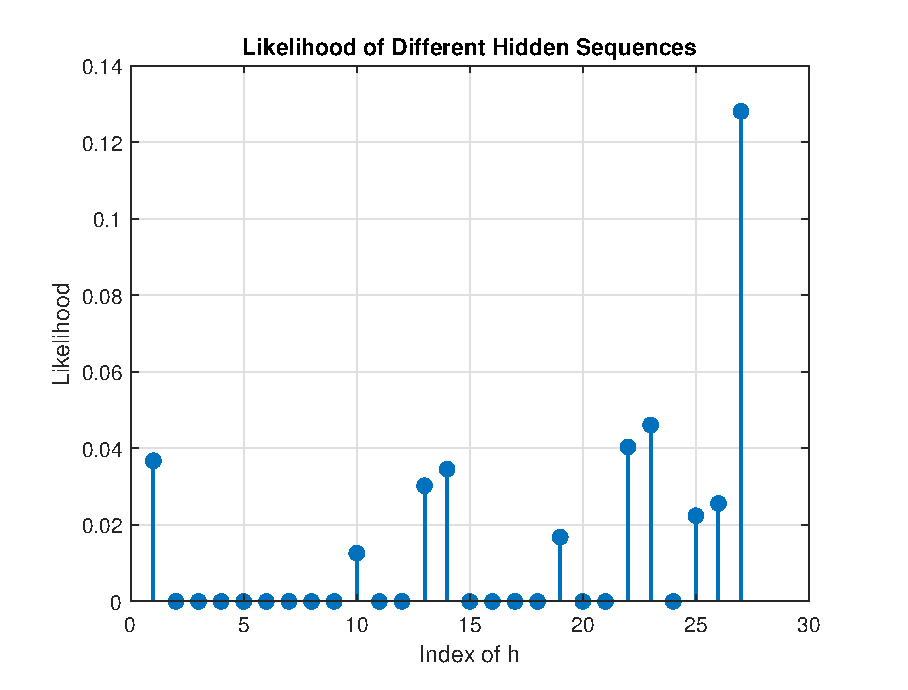
\includegraphics[width=0.8\textwidth]{HW8_P1_likelihoods.eps}     
    \caption{Stem plot for all possible states of $h_{1:3}$}
    % \label{fig:eps-figure}
\end{figure}

% Note that for many state sequences $h_{1:3}$ the likelihood is zero, which is expected since by observing $A$ it is clear that from state 2 it can not go to state 1 and similarly from state 3 it can not go to either state 1 or 2.

Note that for many state sequences $h_{1:3}$, the likelihood is zero. This is expected because, as observed in $A$, state 2 cannot transition to state 1, and similarly, state 3 cannot transition to either state 1 or state 2.


\section*{Problem 2}

Suppose the HMM transition matrix \( A \) and emission matrix \( B \) are initialized to uniform values:

\[
A_{ij} = \frac{1}{N}, \quad \forall i, j
\]

where \( N \) is the number of hidden states, ensuring that \( A \) is a valid stochastic matrix. Similarly, let

\[
B_{jk} = \frac{1}{M}, \quad \forall j, k
\]

where \( M \) is the number of observation symbols.

\textbf{E-Step:} The EM algorithm computes expected counts based on current parameters. Since all transition and emission probabilities are equal, the forward and backward probabilities computed during the E-step will also be uniform across states.

\textbf{M-Step:} The parameter $A$ is updated as:

\[
A_{ij}^{\text{new}} = \frac{\sum_t \gamma_t(i, j)}{\sum_t \gamma_t(i)}
\]

where \( \gamma_t(i, j) \) is the expected count of transition \( i \to j \). Since the initialization is uniform, the expected counts remain uniform, and thus the updates do not change the structure of \( A \) and \( B \).

\textbf{Conclusion:} Since the EM updates preserve the uniformity of the matrices, the algorithm fails to update parameters meaningfully.
The algorithm stagnates,
leading to failure in learning a useful model.





\section*{Problem 3}


\subsection*{1. Probability of Sequence under \( p_{\text{new}} \)}

The probability of the sequence \( S = A, A, G, T, A, C, T, T, A, C, C, T, A, C, G, C \) under the transition matrix \( p_{\text{new}} \) is given by:

\[
P(S | p_{\text{new}}) = p(h_1) \prod_{t=1}^{15} p_{\text{new}}(S_{t+1} | S_t)
\]

where \( p(h_1) \) is the initial probability of being in the first state. Given that it is uniformly distributed among \( A, C, G, T \):

\[
p(h_1) = \frac{1}{4}
\]

To compute the probability of the sequence under \( p_{\text{new}} \), the function \textit{sequence\_prob} was written, which is called from the \textit{HW8\_P3.m} file resulting in:

\[
P(S | p_{\text{new}}) = \frac{1}{4} \prod_{t=1}^{15} p_{\text{new}}(S_{t+1} | S_t) = 8.1781 \cdot 10^{-13}
\]

\subsection*{2. Probability under \( q_{\text{new}} \) and Likelihood Comparison}

Similarly, we compute:

\[
P(S | q_{\text{new}}) = \frac{1}{4} \prod_{t=1}^{15} q_{\text{new}}(S_{t+1} | S_t) = 8.6147  \cdot 10^{-24}
\]

Comparing \( P(S | p_{\text{new}}) \) and \( P(S | q_{\text{new}}) \), we determine that \( S \) has a higher likelihood under \( p_{\text{new}} \) as expected, because using the transition matrix \( p_{\text{new}} \) is more probable the next state to be bigger (the numbers in the sequence increase) whereas with \( q_{\text{new}} \) it is more probable the next state to be smaller. 

\subsection*{3. Maximum Likelihood Estimation with MixMarkov}

The function \texttt{generate\_markov\_samples} was created to:
\begin{itemize}
    \item Generate 100 sequences of length 16 from \( p_{\text{new}} \).
    \item Generate 100 sequences of length 16 from \( q_{\text{new}} \).
    % \item Using , we estimated the Maximum Likelihood parameters.
\end{itemize}

While using the function \texttt{MixMarkov.m} some errors occurred, which prevented from getting the final results.

% Assuming \( H = 2 \), the posterior probability of sequence assignment to Markov chains was analyzed.

\subsection*{4. Hidden Markov Model and Most Likely Sequence}

Given the emission distribution:

\[
p(v = i | h = j) =
\begin{cases} 
0.7 & \text{if } i = j \\
0.1 & \text{if } i \neq j
\end{cases}
\]

we adapted \texttt{demoHMMinferenceSimple.m} to compute the most likely hidden sequences \( h_1^{1:16} \) under both transition matrices. The preferred hidden sequence was determined based on likelihood comparisons. The majority of the time the preferred hidden sequence was from \( p_{\text{new}} \).


\section*{Problem 4}

We are tasked with proving that a suitable value of \(M\) such that 
\[
\frac{p^*(x)}{q(x)} \leq M
\]
is 
\[
M = e^{1 + \frac{\pi^2}{2\sigma^2}} \sqrt{2\pi\sigma^2}.
\]

\subsection*{1. Define \(p^*(x)\) and \(q(x)\)}
The target unnormalized probability density is given as:
\[
p^*(x) = e^{\sin(x)}.
\]
The proposal distribution \(q(x)\) is a Gaussian:
\[
q(x) = \frac{1}{\sqrt{2\pi\sigma^2}} \exp\left(-\frac{x^2}{2\sigma^2}\right).
\]

\subsection*{2. Compute \(\frac{p^*(x)}{q(x)}\)}
The ratio of the unnormalized target density to the proposal density is:
\[
\frac{p^*(x)}{q(x)} = \sqrt{2\pi\sigma^2} \, e^{\sin(x)} \, \exp\left(\frac{x^2}{2\sigma^2}\right).
\]

\subsection*{3. Find an upper bound of \(\frac{p^*(x)}{q(x)}\)}
To find \(M\), we need an upper bound of \(\frac{p^*(x)}{q(x)}\) over all \(x \in [-\pi, \pi]\). 

\begin{itemize}
    \item The term \(e^{\sin(x)}\) achieves its maximum when \(\sin(x) = 1\), which occurs at \(x = \frac{\pi}{2}\). Hence:
    \[
    \max e^{\sin(x)} = e^1.
    \]

    \item The term \(\exp\left(\frac{x^2}{2\sigma^2}\right)\) achieves its maximum when \(x^2\) is maximal in the range \([- \pi, \pi]\), which occurs at \(x = \pm\pi\). Hence:
    \[
    \max \exp\left(\frac{x^2}{2\sigma^2}\right) = \exp\left(\frac{\pi^2}{2\sigma^2}\right).
    \]
\end{itemize}

Thus, an upper bound of \(\frac{p^*(x)}{q(x)}\) is:
\[
M = \sqrt{2\pi\sigma^2} \cdot e^1 \cdot \exp\left(\frac{\pi^2}{2\sigma^2}\right).
\]

Simplify:
\[
M = e^{1 + \frac{\pi^2}{2\sigma^2}} \sqrt{2\pi\sigma^2}.
\]

\subsection*{4. Conclusion}
We have shown that the suitable value of \(M\) is:
\[
M = e^{1 + \frac{\pi^2}{2\sigma^2}} \sqrt{2\pi\sigma^2}.
\]
Which ensures that \(\frac{p^*(x)}{q(x)} \leq M\) for all \(x \in [-\pi, \pi]\).


\begin{figure}[H]
    \centering
    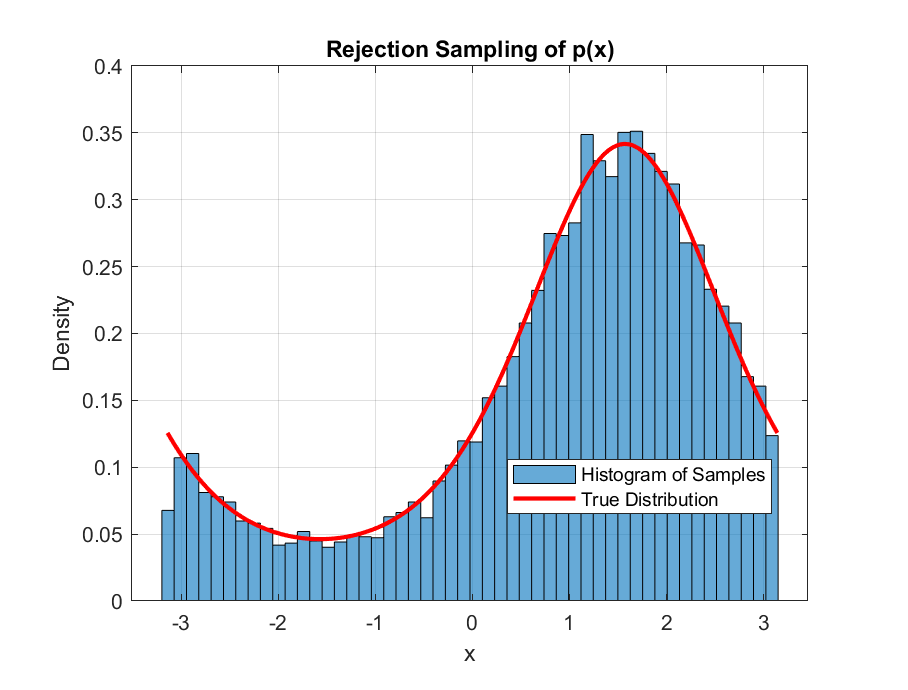
\includegraphics[width=\textwidth]{HW8_P4_rejection_sampling.eps}     
    \caption{Histogram of 10000 samples dawned form $p(x)$}
    % \label{fig:eps-figure}
\end{figure}


\section*{Problem 5}

The original joint distribution is given by
\begin{equation}
    p(x_1, x_2, x_3, x_4, x_5, x_6) = p(x_1)\,p(x_2)\,p(x_3 \mid x_1, x_2)\,p(x_4 \mid x_3)\,p(x_5 \mid x_3)\,p(x_6 \mid x_4, x_5).
\end{equation}

When we fix (or observe) \( x_5 = x_5^* \), the conditional distribution over the remaining variables is
\begin{equation}
\begin{split}
    p(x_1,x_2,x_3,x_4,x_6 \mid x_5 = x_5^*) 
    &= \frac{p(x_1,x_2,x_3,x_4,x_5^*,x_6)}{p(x_5^*)} \\
    &= \frac{p(x_1)\,p(x_2)\,p(x_3\mid x_1,x_2)\,p(x_4\mid x_3)\,p(x_5^*\mid x_3)\,p(x_6\mid x_4,x_5^*)}{p(x_5^*)}.
\end{split}
\end{equation}

Notice that the likelihood term \( p(x_5^*\mid x_3) \) plays a role in the posterior over \( x_3 \).

\subsection*{Ancestral Sampling Procedure}

To sample from \( p(x_1,x_2,x_3,x_4,x_6 \mid x_5 = x_5^*) \), follow these steps:

\begin{enumerate}
    \item \textbf{Sample \(x_1\):} Draw \( x_1 \sim p(x_1) \).
    \item \textbf{Sample \(x_2\):} Draw \( x_2 \sim p(x_2) \).
    \item \textbf{Sample \(x_3\):} Draw \( x_3 \) from 
    \[
    p(x_3\mid x_1,x_2,x_5^*) \propto p(x_3\mid x_1,x_2)\,p(x_5^*\mid x_3).
    \]
    \item \textbf{Sample \(x_4\):} Draw \( x_4 \sim p(x_4\mid x_3) \).
    \item \textbf{Sample \(x_6\):} Draw \( x_6 \sim p(x_6\mid x_4,x_5^*) \).
\end{enumerate}

% This procedure correctly incorporates the evidence \( x_5 = x_5^* \) by adjusting the sampling of \( x_3 \).


% \section*{Setup}

% Assume an HMM with \( N \) states and an observation vocabulary of size \( M \). Let the parameters be initialized as follows:
% \[
% a_{ij} = \frac{1}{N} \quad \text{for all } i,j \quad \text{and} \quad b_{jk} = \frac{1}{M} \quad \text{for all } j,k.
% \]
% Similarly, assume a uniform initial state distribution:
% \[
% \pi_i = \frac{1}{N} \quad \text{for all } i.
% \]

% \section*{Forward--Backward Computation}

% The forward probability at time \( t=1 \) is
% \[
% \alpha_1(i) = \pi_i \, b_i(O_1) = \frac{1}{N} \cdot \frac{1}{M} = \frac{1}{NM}, \quad \text{for each } i.
% \]
% For \( t \ge 1 \), the forward recursion is given by
% \[
% \alpha_{t+1}(j) = \left( \sum_{i=1}^N \alpha_t(i) \, a_{ij} \right) b_j(O_{t+1}).
% \]
% Since \( a_{ij} = \frac{1}{N} \) for all \( i,j \), we have
% \[
% \sum_{i=1}^N \alpha_t(i) \, a_{ij} = \frac{1}{N} \sum_{i=1}^N \alpha_t(i).
% \]
% Notice that the sum \( \sum_{i=1}^N \alpha_t(i) \) is independent of \( j \). Therefore, the term \( \alpha_{t+1}(j) \) becomes
% \[
% \alpha_{t+1}(j) = \frac{1}{N} \left( \sum_{i=1}^N \alpha_t(i) \right) \cdot \frac{1}{M},
% \]
% which is the same for all \( j \). A similar argument applies to the backward probabilities \( \beta_t(i) \). Thus, the smoothed (posterior) state probabilities,
% \[
% \gamma_t(i) = \frac{\alpha_t(i) \beta_t(i)}{\sum_{j=1}^N \alpha_t(j) \beta_t(j)},
% \]
% are uniform in \( i \).

% Likewise, the joint probability of being in state \( i \) at time \( t \) and state \( j \) at time \( t+1 \) is given by
% \[
% \xi_t(i,j) = \frac{\alpha_t(i) \, a_{ij} \, b_j(O_{t+1}) \, \beta_{t+1}(j)}{P(O)},
% \]
% and because \( \alpha_t(i) \), \( a_{ij} \), \( b_j(O_{t+1}) \), and \( \beta_{t+1}(j) \) are all uniform (or constant with respect to the states), the value of \( \xi_t(i,j) \) does not depend on \( i \) or \( j \).

% \section*{EM Re-estimation}

% The EM algorithm re-estimates the parameters by computing expected counts. For the transition probabilities, the re-estimation formula is
% \[
% \hat{a}_{ij} = \frac{\sum_{t=1}^{T-1} \xi_t(i,j)}{\sum_{t=1}^{T-1} \gamma_t(i)}.
% \]
% Since \(\xi_t(i,j)\) is the same for all \( i \) and \( j \) (i.e., it is uniformly distributed), it follows that
% \[
% \hat{a}_{ij} = \frac{1/N}{1} = \frac{1}{N}.
% \]
% Thus, the updated transition probability remains \(\frac{1}{N}\) for every \( i,j \).

% Similarly, the re-estimation of the emission probabilities is given by
% \[
% \hat{b}_j(k) = \frac{\sum_{t=1}^T \mathbb{I}\{O_t = k\} \gamma_t(j)}{\sum_{t=1}^T \gamma_t(j)}.
% \]
% Since \(\gamma_t(j)\) is uniform over \( j \), we obtain
% \[
% \hat{b}_j(k) = \frac{\text{(constant for all } k\text{)}}{\text{(same constant)} } = \frac{1}{M}.
% \]

% \section*{Conclusion}

% When both \( A \) and \( B \) are initialized to uniform values, the forward--backward procedure yields uniform posterior probabilities \(\gamma_t(i)\) and \(\xi_t(i,j)\). Consequently, the re-estimation formulas for both the transition matrix and the emission matrix produce the same uniform values. In other words, the EM algorithm fails to update the parameters meaningfully beyond the initial uniform assignment.




\end{document}
